\newline 
\newline 
\title{LEZIONE 5 17/03/2020}\newline
\textbf{link} \href{https://web.microsoftstream.com/video/72b5f396-c34b-4ff6-8d6e-44bf6832dd2e?list=user&userId=faa91214-a6f5-40d7-8875-253fd49b8ce1}{clicca qui}
\subsubsection*{Esempi}
\textbf{es.} Prendiamo un polinomio caratteristico $\Pi(s) = 5 s^2 +s$: questo è chiaramente non asintoticamente stabile (c'è una radice nulla).\newline
\rule{\textwidth}{0,4pt}\newline
\newline
\textbf{es.} $\Pi(s) = s^3 -s^2 +s +4$: anche questo non è asintoticamente stabile (c'è un coefficiente discorde)\newline
\rule{\textwidth}{0,4pt}\newline
\newline
\textbf{es.} $\Pi(s) = s^5 +4 s^3 +3s^2 +s + 5$: anche questo non è asintoticamene stabile (manca il termine $s^4$ che quindi ha coefficiente nullo).\newline
\rule{\textwidth}{0,4pt}\newline
\newline
\textbf{es.} $\Pi(s) = s^4 +2s^3+4s^2+s+5$: in questo esempio le condizioni necessarie sono soddisfatte, ma non sappiamo dire se è o meno asintoticamente stabile. Ci serve ora un criterio per stabilire se è asintoticamente stabile.\newline
\rule{\textwidth}{0,4pt}
\subsubsection{Criterio di stabilità secondo Routh (SD LTI a TC)}
Il criterio di Routh è una condizione necessaria e succificiente per la stabilità asintotica di un SD LTI a TC (NOTA BENE: \textbf{non vale per sistemi a tempo discreto}! L'analogo a TD è il criterio di Jury, ma noi non lo tratteremo).\newline
\newline
Il criterio di Routh si basa sulla tabella di Routh che si costruisce a partire dal polinomio caratteristico $\Pi(s)$.
\subsubsection*{Tabella di Routh}
Definiamo il polinomio caratteristico come
\[
    \Pi(s) = a_0s^n + a_1 s^{n-1} + \dots + a_{n-1}s + a_n
\]
\textbf{oss.} il polinomio deve avere tutti i termini, altrimenti violiamo una delle condizioni necessarie esposta nella sezione precedente "Criteri di stabilità dedotti dalla matrice A", e il sistema non è sicuramente asintoticamente stabile.\newline
\newline
La tabella di Routh si costruisce nel seguente modo:
\begin{itemize}
    \item Si compilano le prime due righe a "zig-zag" (come mostrato dalle frecce) con i coefficienti del polinomio.
    \[
        \begin{matrix}
            a_0 & \;\;\;\;\;\; a_2 & \;\;\;\;\;\;\dots\\
            \;\;\downarrow & \nearrow \;\; \downarrow & \nearrow \;\; \downarrow\\
            a_1 & \;\;\;\;\;\; a_3 & \;\;\;\;\;\;\dots 
        \end{matrix}
    \]
    \item a seconda che il numero di termini sia pari (le due righe sono di pari lunghezza) o dispari (la prima riga ha un termine in più della seconda, per cui si aggiunge uno $0$) l'ultima colonna può terminare in due modi:
    \[
        \begin{matrix}
            \dots & a_{n-1}\\
            \;\\
            \dots & a_n
        \end{matrix}\;\;\;\;\;\;\;\;\;\;\; \text{oppure}\;\;\;\;\;\;\;\;\;\;\; \begin{matrix}
            \dots &a_n\\
            \;\\
            \dots & 0 
        \end{matrix}
    \]
    \item In totale, considerando anche le prime due righe, ci sono $n+1$ righe.\newline
    Ogni riga dalla terza in poi dipende dalle due precedenti seguendo una regola:
    \[
        \begin{matrix}
            h_1 & h_2 & h_3 &\dots\\
            \;\\
            q_1 & q_2 & q_3 & \dots\\
            \;\\
            w_1 & w_2 & w_3 & \dots
        \end{matrix}
    \]
    prese due generiche righe ($h_i$ e $q_i$), i termini della riga successiva ($w_i$) si costruiscono come $w_i = - \frac{1}{q_1} det\left[\begin{matrix}
        h_1 & h_{i+1} \\
        q_1 & q_{i+1}
    \end{matrix}\right]$.\newline
    Se manca un termine in una delle righe precedenti ($h$ e $q$) si assume nullo.
    \item Se troviamo un elemento nullo in prima colonna, ci si ferma, sicuramente il sistema non è asintoticamente stabile, e siamo in presenza di un caso particolare che non ci permette di calcolare la tabella di Routh.
\end{itemize}
\subsubsection*{Criterio di Routh}
Un sistema dinamico con polinomio caratteristico $\Pi(s)$ è asintoticamente stabile se e solo se tutti gli elementi della prima colonna della tabella di Routh sono concordi (e non nulli).\newline
\newline
\textbf{Corollario}: Se non vi sono elementi nulli in prima colonna, allora il numero di inversioni di segno sulla prima colonna è uguale al numero di radici di $\Pi(s)$ con $Re>0$. [non lo useremo mai questo corollario].
\subsubsection*{Esempi}
\textbf{es.} $\Pi(s) = s^4 + 2s^3 + 4s^2 + s + 5$: soddisfa le condizioni necessarie, quindi faciamo la tabella di Routh. Siccome $n=4$ la tabella avrà $n+1 = 5$ righe:
\[
    \begin{matrix}
        1 & 4 & 5 \\
        2 & 1 & 0 \\
        \alpha & \beta\\
        \gamma\\
        \delta
    \end{matrix} \;\;\;\;\;\;\;\;\;\;\;\;\;\;\;\;\;\;\;\;\alpha = - \frac{1}{2}det\left[\begin{matrix}
        1&4\\2&1
    \end{matrix}\right] = \frac{7}{2}
\]
\[
     \beta = - \frac{1}{2}det\left[\begin{matrix}
        1&5\\2&0
    \end{matrix}\right]=5 \;\;\;\;\; \gamma= -\frac{1}{\alpha} det \left[\begin{matrix}
        2&1\\\alpha&\beta
    \end{matrix}\right] = - \frac{13}{7} \;\;\;\;\; \delta = - \frac{1}{\gamma} det \left[\begin{matrix}
        \alpha & \beta \\ \gamma &0
    \end{matrix}\right]
\]
Siccome $\gamma$ è discorde, sappiamo che non è asintoticamente stabile.\newline
Inoltre fra $\alpha$ e $\gamma$ c'è un'inversione di segno e fra $\gamma$ e $\delta$ c'è un'altra inversione di segno. Avendo due inversioni di segno, so che ci sono due radici con $Re > 0$.\newline
\newline
\textbf{oss.} Da notare che, anche se abbiamo un solo elemento discorde, ci sono due inversioni di segno.\newline
\rule{\textwidth}{0,4pt}\newline
\newline
\textbf{es.} Dato il SD LTI a TC con polinomio caratteristico $\Pi(s) = s^3 + 2s^2 + hs +k$, dire per quali valori di $(h,k)$ esso è asintoticamente stabile.\newline
Deduciamo che dovremo avere $h>0$ e $k>0$ (altrimenti violo una delle condizioni necessarie). Usiamo ora Routh, l'unico caso in cui si può evitare di usare Routh è se il polinomio caratteristico è di secondo grado.
\[
    \begin{matrix}
        1&h\\
        2&k\\
        \alpha\\
        \beta
    \end{matrix} \;\;\;\;\;\;\;\;\;\;\;\;\;\;\;\alpha = - \frac{1}{2}det \left[\begin{matrix}
        1&h\\2&k
    \end{matrix}\right] = \frac{2h-k}{2} \;\;\;\;\;\;\;\;\;\;\;\;\;\;\; \beta = - \frac{1}{\alpha} det \left[\begin{matrix}
        2 & k \\ \alpha & 0
    \end{matrix}\right] = k
\]
Disequazioni per imporre che i termini della prima colonna siano concordi:
\[
    \begin{cases}
        h - \frac{k}{2}>0\\
        k>0
    \end{cases} \Rightarrow \begin{cases}
        k>0\\
        k>2h
    \end{cases} \text{ricordando che} \; k>0 \;\text{e}\;h>0
\]
\rule{\textwidth}{0,4pt}
\newpage
\section{Segnali e trasformate}
Consideriamo un sistema $S$ dinamico LTI a TC (SISO), con un ingresso $u$ e un'uscita $y$.\newline
\newline
[immagine dagli appunti del prof]
\begin{center}
    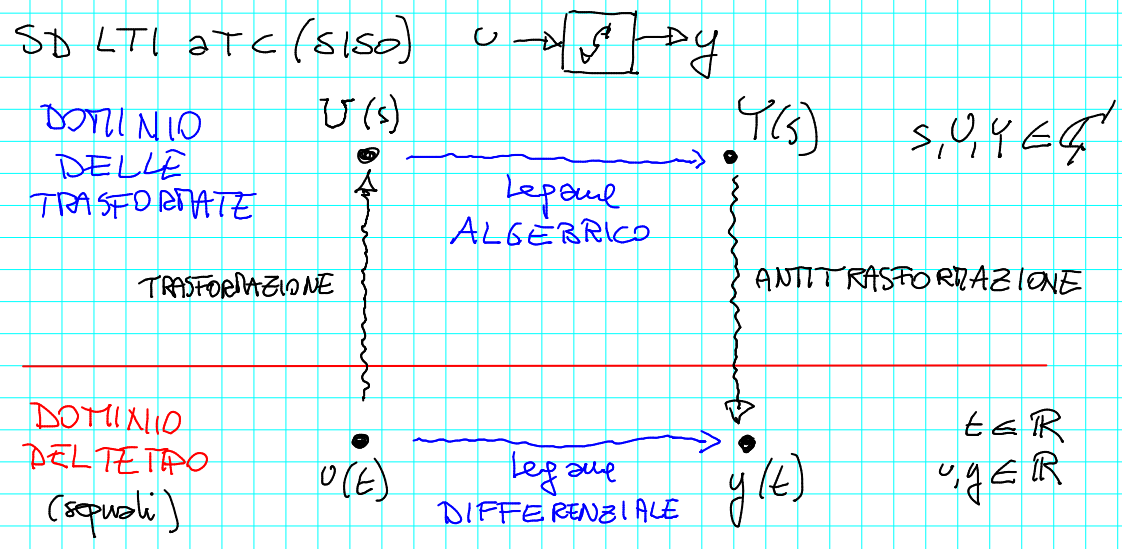
\includegraphics[height=6cm]{../lezione5/img1.PNG}
\end{center}

\textbf{Dominio del tempo}: fra il segnale $u(t)$ (la causa) e il segnale $y(t)$ (l'effetto) nel dominio del tempo c'è un legame differenziale ($u(t) \rightarrow y(t)$). Ciò che attribuisce a un sistema il carattere dinamico è la presenza di equazioni differenziali. Nel dominio del tempo abbiamo $t,u,y \in \mathbb{R}$\newline
\newline
\textbf{Dominio delle trasformate}: Supponiamo di poter associare a $u(t)$ del dominio del tempo, con un operazione che chiamiamo "trasformazione", un'altra funzione $U(s)$ del dominio delle trasformate ($u(t) \rightarrow U(s)$), dove $U$ è una funzione e $s$ è una variabile complessa. Nel dominio delle trasformate fra il segnale $U(s)$ (la causa) e il segnale $Y(s)$ (l'effetto) c'è un legame algebrico ($U(s) \rightarrow  Y(s)$). Facciamo ora l'operazione opposta alla trasformazione con $Y(s)\rightarrow y(t)$, questa operazione prende il nome di "antitrasformazione". Nel dominio delle trasformate abbiamo $s, U ,Y \in \mathbb{C}$.\newline
\newline
Date queste premesse, il legame fra $U(s)$ e $Y(s)$, il cui corrispondente nel dominio del tempo è \textbf{differenziale}, nel dominio delle trasformate è di tipo \textbf{algebrico}.
\subsection{Serie di Fourier}
Dato un segnale $v(t)$ periodico di periodo $T$, posso esprimerlo come 
\[
    v(t)= v_0 + \sum_{k=1}^{\infty} v_k sin(k \omega_0 t + \phi_k)
\]
dove $\omega_0 = \frac{2\pi}{T}$. Questo significa che posso esprimere un segnale periodico come somma di infinite (infinito numerabile) sinusoidi di frequenze multiple di una fondamentale ($\omega_0$, di periodo $T$).
\subsection{Trasformata di Fourier}
Dato un segnale $v(t)$ definito su tutto $\mathbb{R}$ (non necessariamente periodico), chiamiamo la sua \textbf{trasformata di Fourier} il termine 
\[
    V(j \omega) = \mathcal{F}[v(t)] = \int_{-\infty}^{+\infty} v(t) e^{-j \omega t} dt \;\;\;\;\;\text{(se esiste)}\;
\]
L'\textbf{antitrasformata di Fourier}, invece, è
\[
    v(t) = \mathcal{F}^{-1}[V(j \omega)] = \frac{1}{2\pi j} \int_{-\infty}^{+\infty} V(j \omega) e^{j \omega t} d \omega
\]
\textbf{oss.} una trasformata è definita dal suo \textbf{nucleo}, che è $e^{-j \omega t}$.\newline
\newline
\textbf{oss.} l'antitrasformata è un integrale sulla variabile $\omega$. L'integrale viene solitamente introdotto ad analisi 1 con il concetti di somme parziali (\dots per calcolare l'area sottesa a una funzione, si fanno i tipici rettangolini e si sommano, poi si fa tendere l'ampiezza dei rettangolini a zero\dots). Immaginiamo di fare tanti rettangolini dell'asse delle $\omega$, prendiamo uno di questi rettangolini e il suo contributo a $v(t)$ nell'antitrasformata è $e^{j \omega t}$ moltiplicata per un numero complesso $V(j \omega )$. Il termine $e^{j \omega t}$, il nostro nucleo, può avere due aspetti, se $\omega= 0$ è una costante, altrimenti se $omega \neq 0$ è una sinusoide (in realtà sarebbe un numero complesso, ma ricordiamo che un numero complesso può essere espresso come somma di seni e coseni). Ora prendiamo il caso in cui il nucleo è una sinusoide, moltiplicarla per un numero complesso $V(j \omega)$ significa attenuarla o amplificarla (modulo) e sfasarla (argomento). Quindi noi per ricostruire $v(t)$ con l'antitrasformata dobbiamo sommare infinite sinusoidi, ognuna delle quali caratterizzate da una propria ampiezza e una propria fase indicata dal valore di $V(j \omega)$, \textbf{cioè $V(j \omega)$ ci dice quanto pesa ogni frequenza in $v(t)$}. In questo caso $v(t)$ è somma di infinte (infinito del continuo) sinusoidi.
\subsection{Trasformata di Laplace}
Dato un segnale $v(t)$ definito per $t\geq 0$ (o equivalentemente nullo per $t < 0$), definiamo trasformata di Laplace il termine
\[
    V(s) = \mathcal{L}[v(t)] = \int_{0}^{\infty} v(t) e^{-st}dt
\]
con $s,V \in \mathbb{C}$.\newline
L'antitrasformata di Laplace, invece, è
\[
    v(t) = \mathcal{L}^{-1}[V(s)] = \frac{1}{2\pi j} \int_{\alpha + j \infty}^{\alpha - j \infty} V(s) e^{st}ds
\]
dove gli estremi dell'integrale rappresentano il fatto che quanto integriamo rispetto a una variabile complessa ($s$) dobbiamo specificare su quale linea si muove la variabile: la variabile di integrazione $s$ si muove su una retta parallela all'asse immaginario di parte reale (ascissa) $\alpha$, andando con la sua parte immaginaria (ordinata) da $- \infty$ a $+ \infty$.\newline
\newline
\textbf{oss.} Per le trasformate di Laplace il \textbf{nucleo} è $e^{st} = e^{(\alpha + j \omega) t} = e^{\alpha t} (cos(\omega t) + j sin(\omega t))$. Con questa forma di nucleo si possono rappresentare molti più segnali rispetto al nucleo di Fourier. Con il nucleo di Fourier si potevano rappresentare solo le costanti e le sinusoidi, mentre con il nucleo di Laplace anche le sinusoidi che si smorzano, le sinusoidi che divergono, i segnali che esponenzialmente divergono e i segnali che esponenzialmente convergono.\newline
I segnali che si lasciano trasformare secondo Fourier, sono i segnali che si lasciano ricostruire per mezzo di una somma infinita di segnali che partono dal nucleo $e^{j \omega t}$ (costanti e sinusoidi) moltiplicato per un numero complesso $V(j \omega)$ (amplificate o attenuate, e sfasate).\newline
I segnali che si lasciano trasformare secondo Laplace, sono molti di più, perchè il nucleo di partenza $e^{st}$ rappresenta un insieme di segnali molto più grande. Tutti i segnali trasformabili secondo Fourier sono trasformabili anche secondo Laplace, ma non vale il viceversa.\newline
\newline
\textbf{oss.} (Errore tipico) Per trasformare secondo Laplace il termine $\mathcal{L}[v(t-\tau)]$ dobbiamo scrivere $\int_{0}^{\infty}v(t-\tau) e^{-st}dt$. Se avessimo scritto $\mathcal{L}[v(t-\tau)]= \int_{0}^{\infty}v(t-\tau) e^{-s(t-\tau)}$ non avremmo applicato correttamente la definizione di trasformata: il termine $e^{-st}dt$ nell'integrale è sempre fatto così, non va modificato mai, dobbiamo vedere la trasformata di Laplace come un "modulo da compilare": $\mathcal{L}[\_\_] = \int_{0}^{\infty}\_\_ \; e^{-st}dt$.
\subsubsection*{Riassunto dei concetti chiave introdotti}
\begin{itemize}
    \item Le trasformate sono strumenti che legano biunivocamente sengali nel tempo a funzioni complesse di variabile complessa.
    \item Le trasformate di Fourier interpretano un segnale come somma di infinite sinusoidi, invece le trasformate di Laplace non considera sinusoidi, ma delle esponenziali complesse (categoria nella quale rientrano anche le sinusoidi).
\end{itemize}
\subsubsection{Esempi}
Vediamo tre trasformate di Laplace notevoli (da imparare a memoria, useremo praticamente solo queste!).\newline
\newline
\textbf{es.} $v(t) = sca(t) := \begin{cases}
    1 \;\;\;\; &t\geq\\ 0 &t<0 
\end{cases}$, la trasformata di Laplace è
\[
    \mathcal{L}[sca(t)] = \int_{0}^{\infty} sca(t)e^{-st} dt = \int_{0}^{\infty} 1 \cdot e^{-st}dt = \left[\frac{e^{-st}}{-s}\right]_0^\infty = 0 - \frac{1}{-s} = \frac{1}{s}
\]
\rule{\textwidth}{0,4pt}\newline
\newline
\textbf{es.} $v(t) = imp(t) := \begin{cases}
    imp(t)=0 \;\;\;&\forall\;t \neq 0\\
    \int_{-\infty}^{\infty}imp(t) dt =1
\end{cases}$\newline
[immagine dagli appunti del prof]
\begin{center}
    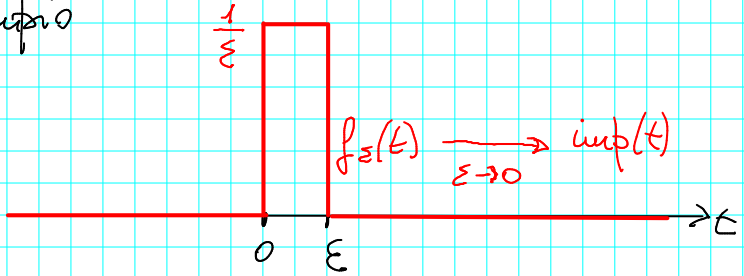
\includegraphics[height=3cm]{../lezione5/img2.PNG}
\end{center}

La trasformata di Laplace è
\[
    \mathcal{L}[imp(t)] = \lim_{\epsilon\rightarrow 0} \mathcal{L}[f_\epsilon(t)] = \lim_{\epsilon\rightarrow 0}\int_{0}^{\infty}f_\epsilon (t) e^{-st} dt = \lim_{\epsilon\rightarrow 0}\int_{0}^{\epsilon}\frac{1}{\epsilon}e^{-st}dt =
\]
\[
    = \lim_{\epsilon\rightarrow 0}\left[\frac{e^{-st}}{-s\epsilon}\right]_0^\epsilon = \lim_{\epsilon\rightarrow 0}\left( \frac{e^{-s\epsilon}}{-s\epsilon}- \frac{1}{-s\epsilon} \right) = \lim_{\epsilon\rightarrow 0} \frac{1- e^{-s \epsilon}}{s\epsilon} = [F.I., Hopital] = \lim_{\epsilon\rightarrow 0}\frac{\cancel{s}e^{-s\epsilon}}{\cancel{s}} = 1
\]
\rule{\textwidth}{0,4pt}\newline
\newline
\textbf{es.} $v(t) = e^{at}$ per $t\geq 0$ o equivalentemente $v(t) = e^{at} sca(t)$, la trasformata di laplace è
\[
    \mathcal{L}[e^{at} sca(t)] = \int_{0}^{\infty}e^{at}e^{-st}dt = \int_{0}^{\infty}e^{(a-s)t}dt = \left[\frac{e^{(a-s)t}}{a-s}\right]_0^\infty = \frac{1}{s-a} \;\;\;\text{se $Re(a-s)<0$, cioè $Re(s)>a$}\;
\]
\rule{\textwidth}{0,4pt}
\subsubsection{Proprietà della trasformata di Laplace}
\begin{itemize}
    \item La trasformata di Laplace è un operatore lineare:
    \[
        \mathcal{L}[\alpha v_1(t) + \beta v_2(t)] = \alpha \mathcal{L}[v_1(t)] + \beta \mathcal{L}[v_2(t)]
    \]
    \item Trasformata di Laplace della derivata: 
    \[
        \mathcal{L}\left[\frac{dv(t)}{dt}\right] = s \mathcal{L}[v(t)]-v(0)
    \] dove se $v$ è discontinua in $0$ si può usare $0^-$.\newline
    Questa proprietà fa si che legami differenziali diventino legami algebrici. L'operazione che nel dominio del tempo è la derivata, corrisponde nel dominio delle trasformate a una moltiplicazione per $s$ e alla differenza di un termine $v(0)$.\newline
    \newline
    \textbf{es.} $\mathcal{L}\left[\frac{d}{dt}sca(t)\right] = s \mathcal{L}[sca(t)] - sca(0^-) = s \frac{1}{s}-0 = 1$.
    \item Trasformata di laplace dell'intergrale:
    \[
        \mathcal{L}\left[\int_{0}^{t}v(\tau)d \tau\right] = \frac{1}{s} \mathcal{L}[v(t)]
    \]
    L'intergale nel dominio del tempo corrisponde a una divisione per $s$ nel dominio delle trasformate.
    \item Trasforamta di Laplace di un segnale ritardato:
    \[
        \mathcal{L}[v(t-\tau)] = e^{-s \tau} \mathcal{L}[v(t)]
    \] con $\tau > 0$ detto ritardo.\newline
    \textbf{dim.} $\mathcal{L}[v(t-\tau)] = \int_{0}^{\infty}v(t-\tau) e^{-st}dt$. Facciamo un cambio di variabile $x = t-\tau \Rightarrow \begin{cases}
        t = x + \tau\\ dt = dx
    \end{cases} \;\;\;\begin{cases}
        t=0 \rightarrow x = - \tau\\ t= \infty \rightarrow  x= \infty
    \end{cases}$, quindi $\int_{0}^{\infty}v(t-\tau) e^{-st}dt = \int_{-\tau}^{\infty} v(x) e^{-s(x+ \tau)}dx = \int_{0}^{\infty}v(x) e^{-sx}e^{-s \tau}dx = e^{-sx}\int_{0}^{\infty}v(x)e^{-sx}dx = e^{-s \tau} \mathcal{L}[v(t)]$.
\end{itemize}
\ \newline